\chapter{Background}
\begin{itemize}
\item {\bf Packet filtering}
\url{https://www.youtube.com/watch?v=XHlqIqPvKw8}
\item {\bf Wireshark tutorial}
\url{https://www.youtube.com/watch?v=Lu05owzpSb8}
\item {\bf Art of Packet Analysis}
\url{https://www.youtube.com/watch?v=Qd6uDg9OGxM}
\item {\bf TCP/IP Packet analysis tutorials}
\url{https://www.youtube.com/watch?v=jWJIGqW6PrY&list=PLD57FE11C7A09034F&index=1}
\end{itemize}

\section{Protocols Introduction}
The File Transfer Protocol (FTP) is a standard network protocol used
to transfer computer files from one host to another host over a
TCP-based network, such as the Internet.\cite{10} FTP is built on a
client-server architecture and uses separate control and data
connections between the client and the server. FTP users may
authenticate themselves using a clear-text sign-in protocol, normally
in the form of a username and password, but can connect anonymously if
the server is configured to allow it. For secure transmission that
protects the username and password, and encrypts the content, FTP is
often secured with SSL/TLS (FTPS). SSH File Transfer Protocol (SFTP)
is sometimes also used instead, but is technologically different.

FTP may run in active or passive mode, which determines how the data
connection is established.\cite{11} In both cases, the client creates a TCP
control connection from a random, usually an unprivileged, port N to
the FTP server command port 21. In active mode, the client starts
listening for incoming data connections from the server on port M. It
sends the FTP command PORT M to inform the server on which port it is
listening. By default, M=N. The server then initiates a data channel
to the client from its port 20, the FTP server data port. In
situations where the client is behind a firewall and unable to accept
incoming TCP connections, passive mode may be used. In this mode, the
client uses the control connection to send a PASV command to the
server and then receives a server IP address and server port number
from the server,\cite{11,12} which the client then uses to open a data
connection from an arbitrary client port to the server IP address and
server port number received.\cite{13} Both modes were updated in September
1998 to support IPv6. Further changes were introduced to the passive
mode at that time, updating it to extended passive mode.\cite{14}

The server responds over the control connection with three-digit
status codes in ASCII with an optional text message. For example "200"
(or "200 OK") means that the last command was successful. The numbers
represent the code for the response and the optional text represents a
human-readable explanation or request (e.g. <Need account for storing
file>).\cite{10} An ongoing transfer of file data over the data connection
can be aborted using an interrupt message sent over the control
connection.

\begin{itemize}
\item FTP (File Transfer Protocol)\\
\begin{itemize}
\item Introduction video:\\
\url{http://www.lynda.com/FTP-tutorials/What-FTP/189068/364891-4.html}
\item Standard RFC (Request for Comments): 
\begin{itemize}
\item FTP Security Extensions: RFC 2228\\
\url{http://www.rfc-editor.org/rfc/rfc2228.txt}\\
\item Internationalization of the File Transfer Protocol: RFC 2640\\
\url{http://www.rfc-editor.org/rfc/rfc2640.txt}\\
\item Encryption using KEA and SKIPJACK: RFC 2773\\
\url{http://www.rfc-editor.org/rfc/rfc2773.txt}\\
\item Extensions to FTP: RFC 3659\\
\url{http://www.rfc-editor.org/rfc/rfc3659.txt}\\
\item FTP Command and Extension Registry: RFC 5797\\
\url{http://www.rfc-editor.org/rfc/rfc5797.txt}\\
\item File Transfer Protocol HOST Command for Virtual Hosts: RFC 7151\\
\url{http://www.rfc-editor.org/rfc/rfc7151.txt}\\
\end{itemize}
\end{itemize}
\item ARP (Address Resolution Protocol)\\
\begin{itemize}
\item Introduction video:\\
\url{https://www.youtube.com/watch?v=2ydK33mPhTY}\\
\item Standard RFC (Request for Comments): 
\begin{itemize}
\item IANA Allocation Guidelines for the Address Resolution 
Protocol (ARP): RFC 5494
\url{http://www.rfc-editor.org/rfc/rfc5494.txt}
\item A Reverse Address Resolution Protocol: RFC 903\\
\url{http://www.rfc-editor.org/rfc/rfc903.txt}
\item Inverse Address Resolution Protocol: RFC 2390\\
\url{http://www.rfc-editor.org/rfc/rfc2390.txt}
\item Address Resolution Protocol (ARP) Mediation for IP 
Interworking of Layer 2 VPNs: RFC 6575\\
\url{http://www.rfc-editor.org/rfc/rfc6575.txt}
\item FTP Command and Extension Registry: RFC 5797\\
\url{http://www.rfc-editor.org/rfc/rfc5797.txt}
\item File Transfer Protocol HOST Command for Virtual Hosts: RFC 7151\\
\url{http://www.rfc-editor.org/rfc/rfc7151.txt}
\end{itemize}
\end{itemize}
\item HTTP (Hypertext Transfer Protocol)\\
\begin{itemize}
\item Introduction video:\\
\url{https://www.youtube.com/watch?v=uvSIR2RhdXk}
\item Standard RFC (Request for Comments): \\
\begin{itemize}
\item Character Set and Language Encoding for Hypertext Transfer Protocol 
(HTTP) Header Field Parameters: RFC 5987 \\
\url{http://www.rfc-editor.org/rfc/rfc5987.txt}
\item Use of the Content-Disposition Header Field in the Hypertext Transfer 
Protocol (HTTP): RFC 6266\\
\url{http://www.rfc-editor.org/rfc/rfc6266.txt}
\item Hypertext Transfer Protocol (HTTP/1.1): Message Syntax and Routing: 
RFC 7230\\
\url{http://www.rfc-editor.org/rfc/rfc7230.txt}
\item Hypertext Transfer Protocol (HTTP/1.1): Semantics and Content: RFC 7231\\
\url{http://www.rfc-editor.org/rfc/rfc7231.txt}
\item Hypertext Transfer Protocol (HTTP/1.1): Conditional Requests: RFC 7232\\
\url{http://www.rfc-editor.org/rfc/rfc7232.txt}
\item Hypertext Transfer Protocol (HTTP/1.1): Range Requests: RFC 7233\\
\url{http://www.rfc-editor.org/rfc/rfc7233.txt}
\item Hypertext Transfer Protocol (HTTP/1.1): Caching: RFC 7234\\
\url{http://www.rfc-editor.org/rfc/rfc7234.txt}
\item Hypertext Transfer Protocol (HTTP/1.1): Authentication: RFC 7235\\
\url{http://www.rfc-editor.org/rfc/rfc7235.txt}
\item The Hypertext Transfer Protocol Status Code 308 (Permanent Redirect): 
RFC 7538\\
\url{http://www.rfc-editor.org/rfc/rfc7538.txt}
\item Hypertext Transfer Protocol Version 2 (HTTP/2): RFC 7540\\
\url{http://www.rfc-editor.org/rfc/rfc7540.txt}
\end{itemize}
\end{itemize}
\item HTTPS (Hypertext Transfer Protocol Secure)\\
\begin{itemize}
\item Introduction video:\\
\url{https://www.youtube.com/watch?v=JCvPnwpWVUQ}
\item Standard RFC (Request for Comments): \\
\begin{itemize}
\item Internet Printing Protocol (IPP) over HTTPS Transport Binding 
and the 'ipps' URI Scheme: RFC 7472 \\
\url{http://www.rfc-editor.org/rfc/rfc7472.txt}
\end{itemize}
\end{itemize}
\item SMTP (Simple Mail Transfer Protocol)\\
\begin{itemize}
\item Introduction video:\\
\url{https://www.youtube.com/watch?v=1X3dX2JEhLE}
\item Standard RFC (Request for Comments): \\
\begin{itemize}
\item SMTP Service Extension for Message Size Declaration: RFC 1870\\
\url{http://www.rfc-editor.org/rfc/rfc1870.txt}
\item SMTP Service Extension for Command Pipelining: RFC 2920\\
\url{http://www.rfc-editor.org/rfc/rfc2920.txt}
\item SMTP Service Extension for 8-bit MIME Transport: RFC 6152\\
\url{http://www.rfc-editor.org/rfc/rfc6152.txt}
\item SMTP Service Extension for Remote Message Queue Starting: RFC 1985\\
\url{http://www.rfc-editor.org/rfc/rfc1985.txt}
\item SMTP Service Extension for  Returning Enhanced Error Codes: RFC 2034\\
\url{http://www.rfc-editor.org/rfc/rfc2034.txt}
\item Deliver By SMTP Service Extension: RFC 2852\\
\url{http://www.rfc-editor.org/rfc/rfc2852.txt}
\item SMTP Service Extensions for Transmission of Large and Binary 
MIME Messages: RFC 3030\\
\url{http://www.rfc-editor.org/rfc/rfc3030.txt}
\item SMTP Service Extension for Secure SMTP over Transport Layer 
Security: RFC 3207\\
\url{http://www.rfc-editor.org/rfc/rfc3207.txt}
\item A No Soliciting Simple Mail Transfer Protocol (SMTP) Service 
Extension: RFC 3865\\
\url{http://www.rfc-editor.org/rfc/rfc3865.txt}
\item SMTP Service Extension for Message Tracking: RFC 3885\\
\url{http://www.rfc-editor.org/rfc/rfc3885.txt}
\item SMTP and MIME Extensions for Content Conversion: RFC 4141\\
\url{http://www.rfc-editor.org/rfc/rfc4141.txt}
\item SMTP Submission Service Extension for Future Message Release: RFC 4865\\
\url{http://www.rfc-editor.org/rfc/rfc4865.txt}
\item A Registry for SMTP Enhanced Mail System Status Codes: RFC 5248\\
\url{http://www.rfc-editor.org/rfc/rfc5248.txt}
\item SMTP Extension for Internationalized Email: RFC 6531\\
\url{http://www.rfc-editor.org/rfc/rfc6531.txt}
\item Email Greylisting: An Applicability Statement for SMTP: RFC 6647\\
\url{http://www.rfc-editor.org/rfc/rfc6647.txt}
\item The Require-Recipient-Valid-Since Header Field and SMTP Service 
Extension: RFC 7293\\s
\url{http://www.rfc-editor.org/rfc/rfc7293.txt}
\end{itemize}
\end{itemize}
\item DHCP (Dynamic Host Configuration Protocol)\\ 
\begin{itemize}
\item Introduction video:\\
\url{https://www.youtube.com/watch?v=CgsRdy0iCiE}
\item Standard RFC (Request for Comments): \\
\begin{itemize}
\item Interoperation Between DHCP and BOOTP: RFC 1534\\
\url{http://www.rfc-editor.org/rfc/rfc1534.txt}
\item DHCP Options for Novell Directory Services: RFC 2241\\
\url{http://www.rfc-editor.org/rfc/rfc2241.txt}
\item DHCP Option for The Open Group's User Authentication Protocol: 
RFC 2485\\
\url{http://www.rfc-editor.org/rfc/rfc2485.txt}
\item DHCP Option to Disable Stateless Auto-Configuration in IPv4 
Clients: RFC 2563\\
\url{http://www.rfc-editor.org/rfc/rfc2563.txt}
\item DHCP Options for Service Location Protocol: RFC 2610\\
\url{http://www.rfc-editor.org/rfc/rfc2610.txt}
\item DHCP for IEEE 1394: RFC 2855\\
\url{http://www.rfc-editor.org/rfc/rfc2855.txt}
\item The Name Service Search Option for DHCP: RFC 2937\\
\url{http://www.rfc-editor.org/rfc/rfc2937.txt}
\item The User Class Option for DHCP: RFC 3004\\
\url{http://www.rfc-editor.org/rfc/rfc3004.txt}
\item The IPv4 Subnet Selection Option for DHCP: RFC 3011\\
\url{http://www.rfc-editor.org/rfc/rfc3011.txt}
\item Authentication for DHCP Messages: RFC 3118\\
\url{http://www.rfc-editor.org/rfc/rfc3118.txt}
\item The DOCSIS (Data-Over-Cable Service Interface Specifications) 
Device Class DHCP (Dynamic Host Configuration Protocol) Relay Agent 
Information Sub-option: RFC 3256\\
\url{http://www.rfc-editor.org/rfc/rfc3256.txt}
\item Dynamic Host Configuration Protocol (DHCPv6) Options for Session 
Initiation Protocol (SIP) Servers: RFC 3319\\
\url{http://www.rfc-editor.org/rfc/rfc3319.txt}
\item Dynamic Host Configuration Protocol (DHCP-for-IPv4) Option for 
Session Initiation Protocol (SIP) Servers: RFC 3361\\
\url{http://www.rfc-editor.org/rfc/rfc3361.txt}
\item Encoding Long Options in the Dynamic Host Configuration Protocol 
(DHCPv4): RFC 3396\\
\url{http://www.rfc-editor.org/rfc/rfc3396.txt}
\item Dynamic Host Configuration Protocol (DHCP) Domain Search Option: 
RFC 3397\\
\url{http://www.rfc-editor.org/rfc/rfc3397.txt}
\item The Classless Static Route Option for Dynamic Host Configuration 
Protocol (DHCP) version 4: RFC 3442\\
\url{http://www.rfc-editor.org/rfc/rfc3442.txt}
\item Dynamic Host Configuration Protocol (DHCPv4) Configuration of 
IPsec Tunnel Mode: RFC 3456\\
\url{http://www.rfc-editor.org/rfc/rfc3456.txt}
\item Dynamic Host Configuration Protocol (DHCP) Option for CableLabs 
Client Configuration: RFC 3495\\
\url{http://www.rfc-editor.org/rfc/rfc3495.txt}
\item Link Selection sub-option for the Relay Agent Information 
Option for DHCPv4: RFC 3527\\
\url{http://www.rfc-editor.org/rfc/rfc3527.txt}
\item PacketCable Security Ticket Control Sub-Option for the 
DHCP CableLabs Client Configuration (CCC) Option: RFC 3594\\
\url{http://www.rfc-editor.org/rfc/rfc3594.txt}
\item Key Distribution Center (KDC) Server Address Sub-option for the 
Dynamic Host Configuration Protocol (DHCP) CableLabs Client 
Configuration (CCC) Option: RFC 3634\\
\url{http://www.rfc-editor.org/rfc/rfc3634.txt}
\item Stateless Dynamic Host Configuration Protocol (DHCP) Service for 
IPv6: RFC 3736\\
\url{http://www.rfc-editor.org/rfc/rfc3736.txt}
\item Network Information Service (NIS) Configuration Options for 
Dynamic Host Configuration Protocol for IPv6 (DHCPv6): RFC 3898\\
\url{http://www.rfc-editor.org/rfc/rfc3898.txt}
\item Vendor-Identifying Vendor Options for Dynamic Host Configuration 
Protocol version 4 (DHCPv4): RFC 3925\\
\url{http://www.rfc-editor.org/rfc/rfc3925.txt}
\item Reclassifying Dynamic Host Configuration Protocol version 4 
(DHCPv4) Options: RFC 3942\\
\url{http://www.rfc-editor.org/rfc/rfc3942.txt}
\item Subscriber-ID Suboption for the Dynamic Host Configuration 
Protocol (DHCP) Relay Agent Option: RFC 3993\\
\url{http://www.rfc-editor.org/rfc/rfc3993.txt}
\item Remote Authentication Dial-In User Service (RADIUS) Attributes 
Suboption for the Dynamic Host Configuration Protocol (DHCP) Relay 
Agent Information Option: RFC 4014\\
\url{http://www.rfc-editor.org/rfc/rfc4014.txt}
\item The Authentication Suboption for the Dynamic Host Configuration 
Protocol (DHCP) Relay Agent Option: RFC 4030\\
\url{http://www.rfc-editor.org/rfc/rfc4030.txt}
\item Rapid Commit Option for the Dynamic Host Configuration Protocol 
version 4 (DHCPv4): RFC 4039\\
\url{http://www.rfc-editor.org/rfc/rfc4039.txt}
\item Simple Network Time Protocol (SNTP) Configuration Option for 
DHCPv6: RFC 4075\\
\url{http://www.rfc-editor.org/rfc/rfc4075.txt}
\item Information Refresh Time Option for Dynamic Host Configuration 
Protocol for IPv6 (DHCPv6): RFC 4242\\
\url{http://www.rfc-editor.org/rfc/rfc4242.txt}
\item Vendor-Specific Information Suboption for the Dynamic Host 
Configuration Protocol (DHCP) Relay Agent Option: RFC 4243\\
\url{http://www.rfc-editor.org/rfc/rfc4243.txt}
\item Dynamic Host Configuration Protocol (DHCP) Options for Broadcast 
and Multicast Control Servers: RFC 4280\\
\url{http://www.rfc-editor.org/rfc/rfc4280.txt}
\item Dynamic Host Configuration Protocol (DHCP) over InfiniBand: 
RFC 4390\\
\url{http://www.rfc-editor.org/rfc/rfc4390.txt}
\item Dynamic Host Configuration Protocol for IPv6 (DHCPv6) Relay 
Agent Subscriber-ID Option: RFC 4580\\
\url{http://www.rfc-editor.org/rfc/rfc4580.txt}
\item Dynamic Host Configuration Protocol for IPv6 (DHCPv6) Relay 
Agent Remote-ID Option: RFC 4649\\
\url{http://www.rfc-editor.org/rfc/rfc4649.txt}
\item The Dynamic Host Configuration Protocol (DHCP) Client Fully 
Qualified Domain Name (FQDN) Option: RFC 4702\\
\url{http://www.rfc-editor.org/rfc/rfc4702.txt}
\item Resolution of Fully Qualified Domain Name (FQDN) Conflicts 
among Dynamic Host Configuration Protocol (DHCP) Clients: RFC 4703\\
\url{http://www.rfc-editor.org/rfc/rfc4703.txt}
\item The Dynamic Host Configuration Protocol for IPv6 (DHCPv6) 
Client Fully Qualified Domain Name (FQDN) Option: RFC 4704\\
\url{http://www.rfc-editor.org/rfc/rfc4704.txt}
\item Timezone Options for DHCP: RFC 4833\\
\url{http://www.rfc-editor.org/rfc/rfc4833.txt}
\item DHCPv6 Relay Agent Echo Request Option: RFC 4994\\
\url{http://www.rfc-editor.org/rfc/rfc4994.txt}
\item DHCPv6 Leasequery: RFC 5007\\
\url{http://www.rfc-editor.org/rfc/rfc5007.txt}
\item The Dynamic Host Configuration Protocol Version 4 (DHCPv4) 
Relay Agent Flags Suboption: RFC 5010\\
\url{http://www.rfc-editor.org/rfc/rfc5010.txt}
\item DHCP Server Identifier Override Suboption: RFC 5107\\
\url{http://www.rfc-editor.org/rfc/rfc5107.txt}
\item DHCP Options for Protocol for Carrying Authentication for 
Network Access (PANA) Authentication Agents: RFC 5192\\
\url{http://www.rfc-editor.org/rfc/rfc5192.txt}
\item Discovering Location-to-Service Translation (LoST) Servers 
Using the Dynamic Host Configuration Protocol (DHCP): RFC 5223\\
\url{http://www.rfc-editor.org/rfc/rfc5223.txt}
\item Control And Provisioning of Wireless Access Points (CAPWAP) 
Access Controller DHCP Option: RFC 5417\\
\url{http://www.rfc-editor.org/rfc/rfc5417.txt}
\item DHCPv6 Bulk Leasequery: RFC 5460\\
\url{http://www.rfc-editor.org/rfc/rfc5460.txt}
\item Dynamic Host Configuration Protocol (DHCPv4 and DHCPv6) Options for IEEE 802.21 Mobility Services (MoS) Discovery: RFC 5678\\
\url{http://www.rfc-editor.org/rfc/rfc5678.txt}
\item Network Time Protocol (NTP) Server Option for DHCPv6: RFC 5908\\
\url{http://www.rfc-editor.org/rfc/rfc5908.txt}
\item DHCPv6 Options for Network Boot: RFC 5970\\
\url{http://www.rfc-editor.org/rfc/rfc5970.txt}
\item DHCPv4 Lease Query by Relay Agent Remote ID: RFC 6148\\
\url{http://www.rfc-editor.org/rfc/rfc6148.txt}
\item DHCPv4 and DHCPv6 Options for Access Network Discovery and 
Selection Function (ANDSF) Discovery: RFC 6153\\
\url{http://www.rfc-editor.org/rfc/rfc6153.txt}
\item Lightweight DHCPv6 Relay Agent: RFC 6221\\
\url{http://www.rfc-editor.org/rfc/rfc6221.txt}
\item DHCPv6 Prefix Delegation for Network Mobility (NEMO): RFC 6276\\
\url{http://www.rfc-editor.org/rfc/rfc6276.txt}
\item Dynamic Host Configuration Protocol for IPv6 (DHCPv6) Option for 
Dual-Stack Lite: RFC 6334\\
\url{http://www.rfc-editor.org/rfc/rfc6334.txt}
\item Definition of the UUID-Based DHCPv6 Unique Identifier (DUID-UUID): 
RFC 6355\\
\url{http://www.rfc-editor.org/rfc/rfc6355.txt}
\item Relay-Supplied DHCP Options: RFC 6422\\
\url{http://www.rfc-editor.org/rfc/rfc6422.txt}
\item The EAP Re-authentication Protocol (ERP) Local Domain Name 
DHCPv6 Option: RFC 6440\\
\url{http://www.rfc-editor.org/rfc/rfc6440.txt}
\item Prefix Exclude Option for DHCPv6-based Prefix Delegation: RFC 6603\\
\url{http://www.rfc-editor.org/rfc/rfc6603.txt}
\item Virtual Subnet Selection Options for DHCPv4 and DHCPv6: RFC 6607\\
\url{http://www.rfc-editor.org/rfc/rfc6607.txt}
\item DHCP Options for Home Information Discovery in Mobile IPv6 (MIPv6): RFC 6610\\
\url{http://www.rfc-editor.org/rfc/rfc6610.txt}
\item Rebind Capability in DHCPv6 Reconfigure Messages: RFC 6644\\
\url{http://www.rfc-editor.org/rfc/rfc6644.txt}
\item Kerberos Options for DHCPv6: RFC 6784\\
\url{http://www.rfc-editor.org/rfc/rfc6784.txt}
\item Client Identifier Option in DHCP Server Replies: RFC 6842\\
\url{http://www.rfc-editor.org/rfc/rfc6842.txt}
\item The DHCPv4 Relay Agent Identifier Sub-Option: RFC 6925\\
\url{http://www.rfc-editor.org/rfc/rfc6925.txt}
\item DHCPv4 Bulk Leasequery: RFC 6926\\
\url{http://www.rfc-editor.org/rfc/rfc6926.txt}
\item Client Link-Layer Address Option in DHCPv6: RFC 6939\\
\url{http://www.rfc-editor.org/rfc/rfc6939.txt}
\item Triggering DHCPv6 Reconfiguration from Relay Agents: RFC 6977\\
\url{http://www.rfc-editor.org/rfc/rfc6977.txt}
\item RADIUS Option for the DHCPv6 Relay Agent: RFC 7037\\
\url{http://www.rfc-editor.org/rfc/rfc7037.txt}
\item Distributing Address Selection Policy Using DHCPv6: RFC 7078\\
\url{http://www.rfc-editor.org/rfc/rfc7078.txt}
\item Handling Unknown DHCPv6 Messages: RFC 7283\\
\url{http://www.rfc-editor.org/rfc/rfc7283.txt}
\item DHCP Options for the Port Control Protocol (PCP): RFC 7291\\
\url{http://www.rfc-editor.org/rfc/rfc7291.txt}
\item DHCPv4-over-DHCPv6 (DHCP 4o6) Transport: RFC 7341\\
\url{http://www.rfc-editor.org/rfc/rfc7341.txt}
\item Source Address Validation Improvement (SAVI) Solution for 
DHCP: RFC 7513\\
\url{http://www.rfc-editor.org/rfc/rfc7513.txt}
\item Issues and Recommendations with Multiple Stateful DHCPv6 
Options: RFC 7550\\
\url{http://www.rfc-editor.org/rfc/rfc7550.txt}
\end{itemize}
\end{itemize}
\item SSH (Secure Shell)\\
\begin{itemize}
\item Introduction video:\\
\url{http://www.lynda.com/Developer-Network-Administration-tutorials/What-SSH/189066/365614-4.html}
\item Standard RFC (Request for Comments): \\
\begin{itemize}
\item The Secure Shell (SSH) Protocol Assigned Numbers: RFC 4250\\
\url{http://www.rfc-editor.org/rfc/rfc4250.txt}
\item The Secure Shell (SSH) Protocol Architecture: RFC 4251\\
\url{http://www.rfc-editor.org/rfc/rfc4251.txt}
\item The Secure Shell (SSH) Authentication Protocol: RFC 4252\\
\url{http://www.rfc-editor.org/rfc/rfc4252.txt}
\item The Secure Shell (SSH) Transport Layer Protocol: RFC 4253\\
\url{http://www.rfc-editor.org/rfc/rfc4253.txt}
\item The Secure Shell (SSH) Connection Protocol: RFC 4254\\
\url{http://www.rfc-editor.org/rfc/rfc4254.txt}
\item Using DNS to Securely Publish Secure Shell (SSH) Key Fingerprints: RFC 4255\\
\url{http://www.rfc-editor.org/rfc/rfc4255.txt}
\item Generic Message Exchange Authentication for the Secure Shell Protocol (SSH): RFC 4256\\
\url{http://www.rfc-editor.org/rfc/rfc4256.txt}
\item The Secure Shell (SSH) Session Channel Break Extension: RFC 4335\\
\url{http://www.rfc-editor.org/rfc/rfc4335.txt}
\item The Secure Shell (SSH) Transport Layer Encryption Modes: RFC 4344\\
\url{http://www.rfc-editor.org/rfc/rfc4344.txt}
\item Improved Arcfour Modes for the Secure Shell (SSH) Transport 
Layer Protocol: RFC 4345\\
\url{http://www.rfc-editor.org/rfc/rfc4345.txt}
\item Diffie-Hellman Group Exchange for the Secure Shell (SSH) 
Transport Layer Protocol: RFC 4419\\
\url{http://www.rfc-editor.org/rfc/rfc4419.txt}
\item RSA Key Exchange for the Secure Shell (SSH) Transport Layer 
Protocol: RFC 4432\\
\url{http://www.rfc-editor.org/rfc/rfc4432.txt}
\item Generic Security Service Application Program Interface (GSS-API) 
Authentication and Key Exchange for the Secure Shell (SSH) Protocol: RFC 4462\\
\url{http://www.rfc-editor.org/rfc/rfc4462.txt}
\item Using the NETCONF Protocol over Secure Shell (SSH): RFC 6242\\
\url{http://www.rfc-editor.org/rfc/rfc6242.txt}
\item Use of the SHA-256 Algorithm with RSA, Digital Signature 
Algorithm (DSA), and Elliptic Curve DSA (ECDSA) in SSHFP Resource 
Records: RFC 6594\\
\url{http://www.rfc-editor.org/rfc/rfc6594.txt}
\item SHA-2 Data Integrity Verification for the Secure Shell (SSH) 
Transport Layer Protocol: RFC 6668\\
\url{http://www.rfc-editor.org/rfc/rfc6668.txt}
\end{itemize}
\end{itemize}
\item DNS (Domain Name System)\\
\begin{itemize}
\item Introduction video:\\
\url{https://www.youtube.com/watch?v=486d8jeCK9M}
\item Standard RFC (Request for Comments): \\
\begin{itemize}
\item Automated Updates of DNS Security (DNSSEC) Trust Anchors: RFC 5011\\
\url{http://www.rfc-editor.org/rfc/rfc5011.txt}
\item Extension Mechanisms for DNS (EDNS(0)): RFC 6891\\
\url{http://www.rfc-editor.org/rfc/rfc6891.txt}
\item DNS Extensions to Support IP Version 6: RFC 3596\\
\url{http://www.rfc-editor.org/rfc/rfc3596.txt}
\item Incremental Zone Transfer in DNS: RFC 1995\\
\url{http://www.rfc-editor.org/rfc/rfc1995.txt}
\item DNS Request and Transaction Signatures (SIG(0)s): RFC 2931\\
\url{http://www.rfc-editor.org/rfc/rfc2931.txt}
\item Secure Domain Name System (DNS) Dynamic Update: RFC 3007\\
\url{http://www.rfc-editor.org/rfc/rfc3007.txt}
\item DNS Configuration options for Dynamic Host Configuration Protocol 
for IPv6 (DHCPv6): RFC 3646\\
\url{http://www.rfc-editor.org/rfc/rfc3646.txt}
\item A Method for Storing IPsec Keying Material in DNS: RFC 4025\\
\url{http://www.rfc-editor.org/rfc/rfc4025.txt}
\item Domain Name System (DNS) Case Insensitivity Clarification: RFC 4343\\
\url{http://www.rfc-editor.org/rfc/rfc4343.txt}
\item DNS Security (DNSSEC) Experiments: RFC 4955\\
\url{http://www.rfc-editor.org/rfc/rfc4955.txt}
\item DNS Name Server Identifier (NSID) Option: RFC 5001\\
\url{http://www.rfc-editor.org/rfc/rfc5001.txt}
\item Measures for Making DNS More Resilient against Forged Answers: 
RFC 5452\\
\url{http://www.rfc-editor.org/rfc/rfc5452.txt}
\item Locating IEEE 802.21 Mobility Services Using DNS: RFC 5679\\
\url{http://www.rfc-editor.org/rfc/rfc5679.txt}
\item DNS SRV Resource Records for AFS: RFC 5864\\
\url{http://www.rfc-editor.org/rfc/rfc5864.txt}
\item Domain Name System (DNS) Security Extensions Mapping for the 
Extensible Provisioning Protocol (EPP): RFC 5910\\
\url{http://www.rfc-editor.org/rfc/rfc5910.txt}
\item DNS Zone Transfer Protocol (AXFR): RFC 5936\\
\url{http://www.rfc-editor.org/rfc/rfc5936.txt}
\item DNS Transport over TCP - Implementation Requirements: RFC 5966\\
\url{http://www.rfc-editor.org/rfc/rfc5966.txt}
\item Cryptographic Algorithm Identifier Allocation for DNSSEC: RFC 6014\\
\url{http://www.rfc-editor.org/rfc/rfc6014.txt}
\item IPv6 Router Advertisement Options for DNS Configuration: RFC 6106\\
\url{http://www.rfc-editor.org/rfc/rfc6106.txt}
\item DNS64: DNS Extensions for Network Address Translation from IPv6 
Clients to IPv4 Servers: RFC 6147\\
\url{http://www.rfc-editor.org/rfc/rfc6147.txt}
\item Elliptic Curve Digital Signature Algorithm (DSA) for DNSSEC: 
RFC 6605\\
\url{http://www.rfc-editor.org/rfc/rfc6605.txt}
\item Using DNS SRV to Specify a Global File Namespace with NFS 
Version 4: RFC 6641\\
\url{http://www.rfc-editor.org/rfc/rfc6641.txt}
\item DNAME Redirection in the DNS: RFC 6672\\
\url{http://www.rfc-editor.org/rfc/rfc6672.txt}
\item DNS Security (DNSSEC) DNSKEY Algorithm IANA Registry Updates: 
RFC 6725\\
\url{http://www.rfc-editor.org/rfc/rfc6725.txt}
\item Improved Recursive DNS Server Selection for Multi-Interfaced Nodes: 
RFC 6731\\
\url{http://www.rfc-editor.org/rfc/rfc6731.txt}
\item Multicast DNS: RFC 6762\\
\url{http://www.rfc-editor.org/rfc/rfc6762.txt}
\item DNS-Based Service Discovery: RFC 6763\\
\url{http://www.rfc-editor.org/rfc/rfc6763.txt}
\item Clarifications and Implementation Notes for DNS Security (DNSSEC): 
RFC 6840\\
\url{http://www.rfc-editor.org/rfc/rfc6840.txt}
\item DNS Certification Authority Authorization (CAA) Resource Record: 
RFC 6844\\
\url{http://www.rfc-editor.org/rfc/rfc6844.txt}
\item Applicability Statement: DNS Security (DNSSEC) DNSKEY Algorithm 
Implementation Status: RFC 6944\\
\url{http://www.rfc-editor.org/rfc/rfc6944.txt}
\item Signaling Cryptographic Algorithm Understanding in DNS Security 
Extensions (DNSSEC): RFC 6975\\
\url{http://www.rfc-editor.org/rfc/rfc6975.txt}
\item Location Information Server (LIS) Discovery Using IP Addresses 
and Reverse DNS: RFC 7216\\
\url{http://www.rfc-editor.org/rfc/rfc7216.txt}
\item Adding Acronyms to Simplify Conversations about DNS-Based 
Authentication of Named Entities (DANE): RFC 7218\\
\url{http://www.rfc-editor.org/rfc/rfc7218.txt}
\item Child-to-Parent Synchronization in DNS: RFC 7477\\
\url{http://www.rfc-editor.org/rfc/rfc7477.txt}
\end{itemize}
\end{itemize}
\end{itemize}

\section{Computing the SHA1 Hash in FTP}
\vspace{1mm}
\noindent
The task is to read a file of FTP packets from the FTP transfer of the
file "reference.java". We have to read the bits, strip out the bytes
corresponding to the file, calculate the SHA1 hash of those bytes, and
return the hash.

\noindent
{\bf Description:}
This file implements the Secure Hashing Algorithm 1 as
defined in FIPS PUB 180-1 published April 17, 1995.

The SHA-1, produces a 160-bit message digest for a given
data stream.  It should take about $2^n$ steps to find a
message with the same digest as a given message and
$2^{(n/2)}$ to find any two messages with the same digest,
when $n$ is the digest size in bits.  Therefore, this
algorithm can serve as a means of providing a
``fingerprint'' for a message.

\subsection{Algorithm Description}
\begin{itemize}
\item Padding
\begin{itemize}
\item Pad the message with a single one followed by zeros until the
final block has 448 bits.
\item Append the size of the original message as an unsigned 64-bit
integer
\end{itemize}
\item Initialize the 5 hash blocks (h0,h1,h2,h3,h4) to the specific
constants defined in the SHA1 standard.
\item Hash (for each 512-bit block)
\begin{itemize}
\item Allocate an 80 word array for the message schedule
 \begin{itemize}
 \item Set the first 16 words to be the 512-bit block split into 16 words
 \item The rest of the words are generated using the following algorithm
  \begin{itemize}
  \item word[i-3] XOR word[i-8] XOR word[i-14] XOR word[i-16] 
  \item rotate 1 bit to the left
  \end{itemize}
 \end{itemize}
\item Loop 80 times doing the following (see \ref{sha1pic})
\begin{itemize}
\item Calculate SHAfunction() and the constants K (these are based on
the current round number)
\item e=d
\item d=c
\item c=b (rotated left 30)
\item b=a
\item a=a (rotated left 5) + SHAfunction() + e + k + word[i]
\end{itemize}
\item Add a,b,c,d, and e to the hash output
\end{itemize}
\item Output the concatenation (h0,h1,h2,h3,h4) which is the message digest
\end{itemize}

\begin{figure}[ht!]
\centering
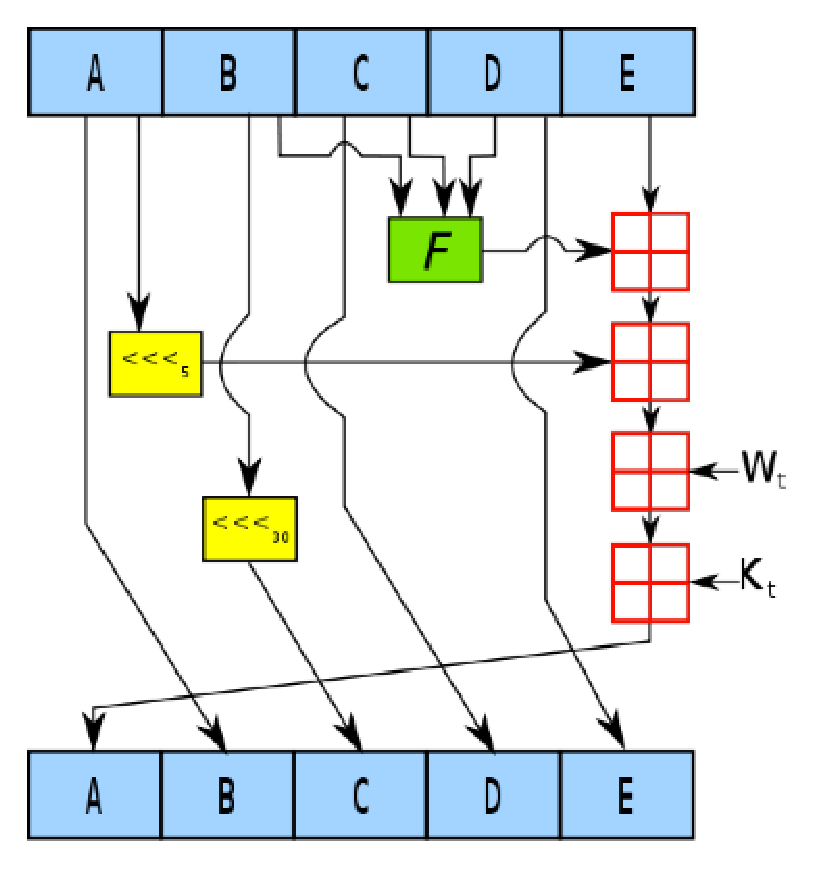
\includegraphics[scale=1.0]{eps/sha1pic.eps}
\caption{The SHA1 computation}
\label{sha1pic}
\end{figure}

\vspace{1mm}
\noindent
{\bf Portability Issues:}
SHA-1 is defined in terms of 32-bit ``words''.  This code
uses \verb|<stdint.h>| (included via ``sha1.h'' to define 32 and 8
bit unsigned integer types.  If your C compiler does not
support 32 bit unsigned integers, this code is not
appropriate.

\vspace{1mm}
\noindent
{\bf Caveats:}
SHA-1 is designed to work with messages less than $2^{64}$ bits
long.  Although SHA-1 allows a message digest to be generated
for messages of any number of bits less than $2^{64}$, this
implementation only works with messages with a length that is
a multiple of the size of an 8-bit character.

\vspace{1mm}
\noindent
See the RFC for SHA1\cite{30} and a video\cite{29} for details.
We use the C code specified in the RFC.

\begin{chunk}{includes}
#include <stdio.h>
#include <fcntl.h>
#include <stdint.h>

\end{chunk}

\begin{chunk}{enums}
enum
{
    shaSuccess = 0,
    shaNull,            /* Null pointer parameter */
    shaInputTooLong,    /* input data too long */
    shaStateError       /* called Input after Result */
};

\end{chunk}

\vspace{1mm}
\noindent
C \#defines
\begin{chunk}{defines}
#define SHA1HashSize 20
#define SHA1CircularShift(bits,word) \
                (((word) << (bits)) | ((word) >> (32-(bits))))


\end{chunk}

\subsection{The SHA1Context struct}
\index{SHA1Context}
\index{struct!SHA1Context}
\noindent
This structure will hold context information for the SHA-1 hashing operation
\begin{chunk}{SHA1Context}
typedef struct SHA1Context
{
 uint32_t Intermediate_Hash[SHA1HashSize/4]; /* Message Digest          */
 uint32_t Length_Low;               /* Message length in bits           */
 uint32_t Length_High;              /* Message length in bits           */
 int_least16_t Message_Block_Index; /* Index into message block array   */
 uint8_t Message_Block[64];         /* 512-bit message blocks           */
 int Computed;                      /* Is the digest computed?          */
 int Corrupted;                     /* Is the message digest corrupted? */
} SHA1Context;

\end{chunk}

\noindent
Function prototypes
\begin{chunk}{prototypes}
int SHA1Reset(  SHA1Context *);
int SHA1Input(  SHA1Context *, const uint8_t *, unsigned int);
int SHA1Result( SHA1Context *, uint8_t Message_Digest[SHA1HashSize]);
void SHA1PadMessage(SHA1Context *);
void SHA1ProcessMessageBlock(SHA1Context *);

\end{chunk}

\subsection{The SHA1Reset function}
\index{SHA1Reset}
\index{function!SHA1Reset}
\noindent
The {\bf SHA1Reset} function will initialize the SHA1Context in preparation
for computing a new SHA1 message digest. It modifies the {\bf context}
structure to contain the initial values.
\begin{chunk}{SHA1Reset}
int SHA1Reset(SHA1Context *context) {
  if (!context) {
    return shaNull;
  }
  context->Length_Low             = 0;
  context->Length_High            = 0;
  context->Message_Block_Index    = 0;
  context->Intermediate_Hash[0]   = 0x67452301;  /* H0 */
  context->Intermediate_Hash[1]   = 0xEFCDAB89;  /* H1 */
  context->Intermediate_Hash[2]   = 0x98BADCFE;  /* H2 */
  context->Intermediate_Hash[3]   = 0x10325476;  /* H3 */
  context->Intermediate_Hash[4]   = 0xC3D2E1F0;  /* H4 */
  context->Computed   = 0;
  context->Corrupted  = 0;
  return shaSuccess;
}

\end{chunk}

\subsection{The SHA1PadMessage function}
\index{SHA1PadMessage}
\index{function!SHA1PadMessage}
For {\bf SHA1PadMessage},the message must be padded to an even
512 bits. The first padding bit must be a '1'.  The last 64
bits represent the length of the original message.  All bits in
between should be 0.  This function will pad the message
according to those rules by filling the Message\_Block array
accordingly.  It will also call the 
{\bf ProcessMessageBlock} [\ref{ProcessMessageBlock}] function
provided appropriately.  When it returns, it can be assumed that
the message digest has been computed.

If the current message block is too small to hold the initial padding
bits and length then we will pad the block, process it, and then
continue padding into a second block.

\begin{chunk}{SHA1PadMessage}
void SHA1PadMessage(SHA1Context *context) {
  if (context->Message_Block_Index > 55) {
    context->Message_Block[context->Message_Block_Index++] = 0x80;
    while(context->Message_Block_Index < 64) {
      context->Message_Block[context->Message_Block_Index++] = 0;
    }
    SHA1ProcessMessageBlock(context);
    while(context->Message_Block_Index < 56) {
      context->Message_Block[context->Message_Block_Index++] = 0;
    }
  } else {
    context->Message_Block[context->Message_Block_Index++] = 0x80;
    while(context->Message_Block_Index < 56) {
     context->Message_Block[context->Message_Block_Index++] = 0;
    }
  }
  /* Store the message length as the last 8 octets */
  context->Message_Block[56] = context->Length_High >> 24;
  context->Message_Block[57] = context->Length_High >> 16;
  context->Message_Block[58] = context->Length_High >> 8;
  context->Message_Block[59] = context->Length_High;
  context->Message_Block[60] = context->Length_Low >> 24;
  context->Message_Block[61] = context->Length_Low >> 16;
  context->Message_Block[62] = context->Length_Low >> 8;
  context->Message_Block[63] = context->Length_Low;
  SHA1ProcessMessageBlock(context);
}

\end{chunk}

\subsection{The SHA1Result function}
\index{SHA1Result}
\index{function!SHA1Result}
The {\bf SHA1Result} will return the 160-bit message digest into the
Message\_Digest array  provided by the caller. 
NOTE: The first octet of hash is stored in the 0th element,
the last octet of hash in the 19th element.
\begin{chunk}{SHA1Result}
int SHA1Result( SHA1Context *context, uint8_t Message_Digest[SHA1HashSize]) {
  int i;
  if (!context || !Message_Digest) {
    return shaNull;
  }
  if (context->Corrupted) {
    return context->Corrupted;
  }
  if (!context->Computed) {
    SHA1PadMessage(context);
    for(i=0; i<64; ++i) {
      context->Message_Block[i] = 0; /* message may be sensitive, clear it */
    }
    context->Length_Low = 0;         /* and clear length */
    context->Length_High = 0;
    context->Computed = 1;
  }
  for(i = 0; i < SHA1HashSize; ++i) {
    Message_Digest[i] = 
      context->Intermediate_Hash[i>>2] >> 8 * ( 3 - ( i & 0x03 ) );
  }
  return shaSuccess;
}

\end{chunk}

\subsection{The SHA1ProcessMessageBlock function}
\label{ProcessMessageBlock}
\index{SHA1ProcessMessageBlock}
\index{function!SHA1ProcessMessageBlock}
The {\bf SHA1ProcessMessageBlock} will process the next 512 bits 
of the message stored in the Message\_Block array.
Note that single character names were used because those were the
names used in the publication.
\begin{chunk}{SHA1ProcessMessageBlock}
void SHA1ProcessMessageBlock(SHA1Context *context) {
  const uint32_t K[] = { 0x5A827999, 0x6ED9EBA1, 0x8F1BBCDC, 0xCA62C1D6 };
                              /* Constants defined in SHA-1  */
  int t;                      /* Loop counter                */
  uint32_t temp;              /* Temporary word value        */
  uint32_t W[80];             /* Word sequence               */
  uint32_t A, B, C, D, E;     /* Word buffers                */
  for(t = 0; t < 16; t++) {
    W[t] = context->Message_Block[t * 4] << 24;
    W[t] |= context->Message_Block[t * 4 + 1] << 16;
    W[t] |= context->Message_Block[t * 4 + 2] << 8;
    W[t] |= context->Message_Block[t * 4 + 3];
  }
  for(t = 16; t < 80; t++) {
    W[t] = SHA1CircularShift(1,W[t-3] ^ W[t-8] ^ W[t-14] ^ W[t-16]);
  }
  A = context->Intermediate_Hash[0];
  B = context->Intermediate_Hash[1];
  C = context->Intermediate_Hash[2];
  D = context->Intermediate_Hash[3];
  E = context->Intermediate_Hash[4];
  for(t = 0; t < 20; t++) {
    temp =  SHA1CircularShift(5,A) + ((B & C) | ((~B) & D)) + E + W[t] + K[0];
    E = D;
    D = C;
    C = SHA1CircularShift(30,B);
    B = A;
    A = temp;
  }
  for(t = 20; t < 40; t++) {
    temp = SHA1CircularShift(5,A) + (B ^ C ^ D) + E + W[t] + K[1];
    E = D;
    D = C;
    C = SHA1CircularShift(30,B);
    B = A;
    A = temp;
  }
  for(t = 40; t < 60; t++) {
    temp = SHA1CircularShift(5,A)+((B & C) | (B & D) | (C & D))+E+W[t]+K[2];
    E = D;
    D = C;
    C = SHA1CircularShift(30,B);
    B = A;
    A = temp;
  }
  for(t = 60; t < 80; t++) {
    temp = SHA1CircularShift(5,A) + (B ^ C ^ D) + E + W[t] + K[3];
    E = D;
    D = C;
    C = SHA1CircularShift(30,B);
    B = A;
    A = temp;
  }
  context->Intermediate_Hash[0] += A;
  context->Intermediate_Hash[1] += B;
  context->Intermediate_Hash[2] += C;
  context->Intermediate_Hash[3] += D;
  context->Intermediate_Hash[4] += E;
  context->Message_Block_Index = 0;
}

\end{chunk}

\subsection{The SHA1Input function}
\index{SHA1Input}
\index{function!SHA1Input}
The {\bf SHA1Input} accepts an array of octets as the next portion
of the message. The {\bf context} contains the SHA context to update.
The {\bf message\_array} contains the array of characters representing 
the next portion of the message. The {\bf length} is the length of
the message\_array.
\begin{chunk}{SHA1Input}
int SHA1Input(SHA1Context    *context,
              const uint8_t  *message_array,
              unsigned       length) {
  if (!length) {
    return shaSuccess;
  }
  if (!context || !message_array) {
    return shaNull;
  }
  if (context->Computed) {
    context->Corrupted = shaStateError;
    return shaStateError;
  }
  if (context->Corrupted) {
     return context->Corrupted;
  }
  while(length-- && !context->Corrupted) {
    context->Message_Block[context->Message_Block_Index++] =
                  (*message_array & 0xFF);
    context->Length_Low += 8;
    if (context->Length_Low == 0) {
      context->Length_High++;
      if (context->Length_High == 0) {
        context->Corrupted = 1;   /* Message is too long */
      }
    }
    if (context->Message_Block_Index == 64) {
      SHA1ProcessMessageBlock(context);
    }
    message_array++;
  }
  return shaSuccess;
}

\end{chunk}

\subsection{The processFile function}
\index{processFile}
\index{function!processFile}
\noindent
The {\bf processFile} function assumes that the files are {\bf open}
for {\bf binary} reading and writing. It copies the bytes. In a
successful copy, {\bf outcount} will end up 0. 
\begin{chunk}{processfile}
int processfile(FILE* input, FILE* output) {
  unsigned char buffer[1024];
  size_t incount;
  size_t outcount;
  do {
    incount = fread(buffer,sizeof(unsigned char),sizeof(buffer),input);
    if (incount) {
      outcount = fwrite(buffer,1,incount,output); 
    } else {
      outcount = 0;
    }
  } while ((incount > 0) && (incount == outcount));
  return outcount;
}

\end{chunk} 

\subsection{The RFC test set}
\index{RFCtest}
\index{function!RFCtest}
\noindent
The {\bf RFCtest} function runs the test code specified in RFC 3174\cite{30}.
This will exercise the SHA-1 code performing the three
tests documented in FIPS PUB 180-1 plus one which calls
SHA1Input with an exact multiple of 512 bits, plus a few
error test checks.
\begin{chunk}{rfctest.c}
#include <string.h>
\getchunk{includes}
\getchunk{enums}
\getchunk{defines}
\getchunk{SHA1Context}
\getchunk{prototypes}
\getchunk{SHA1Reset}
\getchunk{SHA1PadMessage}
\getchunk{SHA1Result}
\getchunk{SHA1ProcessMessageBlock}
\getchunk{SHA1Input}

/* Define patterns for testing */
#define TEST1   "abc"
#define TEST2a  "abcdbcdecdefdefgefghfghighijhi"
#define TEST2b  "jkijkljklmklmnlmnomnopnopq"
#define TEST2   TEST2a TEST2b
#define TEST3   "a"
#define TEST4a  "01234567012345670123456701234567"
#define TEST4b  "01234567012345670123456701234567"
/* an exact multiple of 512 bits */
#define TEST4   TEST4a TEST4b
char *testarray[4] = { TEST1, TEST2, TEST3, TEST4 };
long int repeatcount[4] = { 1, 1, 1000000, 10 };
char *resultarray[4] = {
    "A9 99 3E 36 47 06 81 6A BA 3E 25 71 78 50 C2 6C 9C D0 D8 9D",
    "84 98 3E 44 1C 3B D2 6E BA AE 4A A1 F9 51 29 E5 E5 46 70 F1",
    "34 AA 97 3C D4 C4 DA A4 F6 1E EB 2B DB AD 27 31 65 34 01 6F",
    "DE A3 56 A2 CD DD 90 C7 A7 EC ED C5 EB B5 63 93 4F 46 04 52"
};

int main() {
  SHA1Context sha;
  int i, j, err;
  uint8_t Message_Digest[20];
  for(j = 0; j < 4; ++j) {
    printf( "\nTest %d: %ld, '%s'\n", j+1, repeatcount[j], testarray[j]);
    err = SHA1Reset(&sha);
    if (err) {
      fprintf(stderr, "SHA1Reset Error %d.\n", err );
      break; /* out of for j loop */
    }
    for(i = 0; i < repeatcount[j]; ++i) {
      err = SHA1Input(&sha,
                      (const unsigned char *) testarray[j],
                      strlen(testarray[j]));
      if (err) {
        fprintf(stderr, "SHA1Input Error %d.\n", err );
        break;    /* out of for i loop */
      }
    }
    err = SHA1Result(&sha, Message_Digest);
    if (err) {
      fprintf(stderr,
             "SHA1Result Error %d, could not compute message digest.\n",
             err );
    } else {
      printf("\t");
      for(i = 0; i < 20 ; ++i) {
        printf("%02X ", Message_Digest[i]);
      }
      printf("\n");
    }
    printf("Should match:\n");
    printf("\t%s\n", resultarray[j]);
  }
  /* Test some error returns */
  err = SHA1Input(&sha,(const unsigned char *) testarray[1], 1);
  printf ("\nError %d. Should be %d.\n", err, shaStateError );
  err = SHA1Reset(0);
  printf ("\nError %d. Should be %d.\n", err, shaNull );
  return 0;
}

\end{chunk}

\subsection{The main function}
\index{main}
\index{function!main}
\noindent
The {\bf main} function opens the file, processes it, and exits.
This is the command line entry purely for testing. The full program
will use functions from the API.
\begin{chunk}{sha1.c}

\getchunk{includes}
\getchunk{enums}
\getchunk{defines}
\getchunk{SHA1Context}
\getchunk{prototypes}
\getchunk{SHA1Reset}
\getchunk{SHA1PadMessage}
\getchunk{SHA1Result}
\getchunk{SHA1ProcessMessageBlock}
\getchunk{SHA1Input}
\getchunk{processfile}

int main(int argc, char *argv[]) {
  FILE *input;
  FILE *output;
  int outcount = 0;
  if (argc != 3 || strcmp(argv[1],"--help") == 0) {
    printf("sha1 inputFilename outputFilename");
  }
  if ( (input = fopen(argv[1],"rb")) == NULL) {
    printf("sha1: %s file not found\n",argv[1]);
    return -1;
  }
  if ( (output = fopen(argv[2],"wb")) == NULL) {
    printf("sha1: could not open output file %s\n",argv[2]);
    return -2;
  }
  if ( (outcount = processfile(input,output)) != 0) {
    printf("sha1: binary copy from %s to %s failed\n",argv[1],argv[2]);
    return outcount;
  }
  if (fclose(output)) {
    printf("sha1: could not close %s\n",argv[2]);
    return -3;
  }
  if (fclose(input)) {
    printf("sha1: could not close %s\n",argv[1]);
    return -4;
  }
  return 0;
}

\end{chunk}


